
\section{Écrans 3D}
\subsection{Two-view 3D displays}
\begin{frame}

  \frametitle{Écrans 3D \\Two-view 3D displays} 
  
  \begin{itemize}
  \item Wavelength Selective Displays:
    
    \begin{itemize}
    \item Each eye receives the image intended for it
    \item Images are filtered	
    \end{itemize}
    
    
    
  \item Advantages:
    \begin{itemize} 	
    \item Any color display device can be used to present the stereoscopic
    \end{itemize}
  \item Inconvénient:
    \begin{itemize} 
    \item Each eye is seeing a different color stimulus
    \end{itemize}
  \end{itemize}
  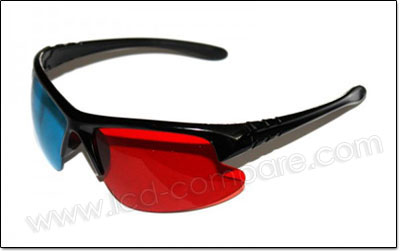
\includegraphics[keepaspectratio,height=.13\linewidth]{1.jpg}
\end{frame}


\begin{frame}		  	
  \begin{itemize}
  \item Time-Sequential Two-View Displays:
    \begin{itemize}
    \item Time-Sequential Polarization:
      \begin{itemize}
      \item Pair of passive polarizing glasses
      \item Each lens is polarized in one direction
      \item The image displayed on the screen is actually composed of two images
      \end{itemize}
    \end{itemize}
  \end{itemize}
  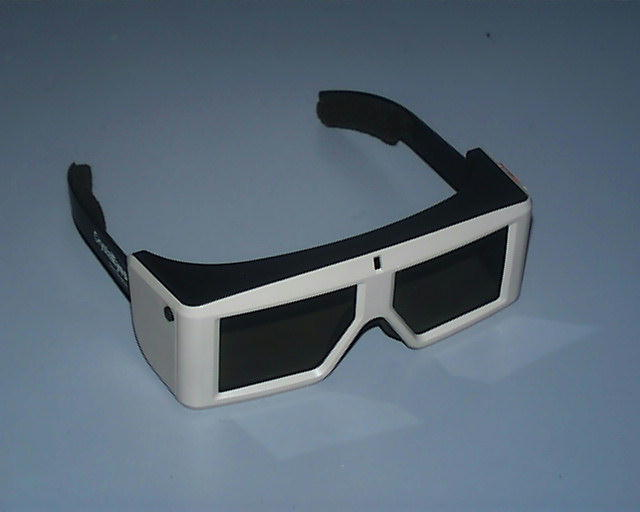
\includegraphics[keepaspectratio,height=.2\linewidth]{2.jpg}
\end{frame}

\begin{frame}
  \begin{itemize}
  \item Time-Sequential Two-View Displays:
    \begin{itemize}
    \item Time-Sequential Backlight:
      \begin{itemize}
      \item Auto-stereoscopic technology
      \item Backlight technique
      \item Having a light source in each side of the screen with a waveguide surface between them.

      \end{itemize}
    \end{itemize}
  \end{itemize}
  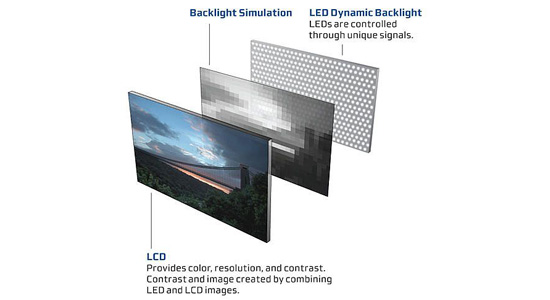
\includegraphics[keepaspectratio,height=.2\linewidth]{3.jpg}
\end{frame}

\subsection{Horizontal parallax multiview 3D displays}	

\begin{frame}

  \frametitle{Écrans 3D \\Horizontal parallax multiview 3D displays} 
  
  \begin{itemize}
  \item Parallax Barrier Displays:
    
    \begin{itemize}
    \item C’est une technique Autostereoscopique.
    \item Elle permet d'obtenir une vision relief sans le port de lunettes.
    \end{itemize}
  \item Les inconvénients:
    \begin{itemize} 	
    \item	Il faut se placer précisément par rapport à l’écran.
    \item Il faut être stable.
    \item Il ne permet pas la visualisation de l’image en relief à plusieurs spectateurs en même temps.
    \end{itemize}
  \end{itemize}
  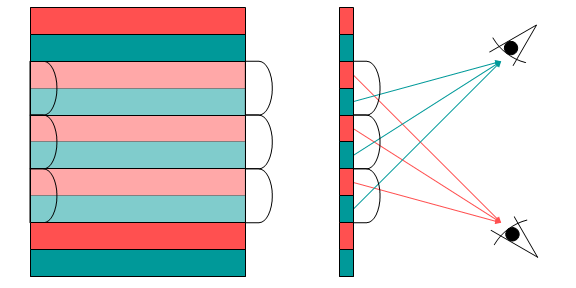
\includegraphics[keepaspectratio,height=.13\linewidth]{4.png}
\end{frame}

\begin{frame}
  \begin{itemize}
  \item Multi-Projector Displays:\\
    Cette technique consiste a positionner en cercle plusieurs vidéo-projecteurs affichant tous un angle d’image différent, apres ces images sont projetées sur un écran spécial. 						
  \item Avantage:
    \begin{itemize} 
    \item Taille de l’image 3D peut être beaucoup plus grande
      il n’est y a pas de limite.
    \end{itemize}
  \item Les inconvénients:
    \begin{itemize} 	
    \item	Plusieurs projecteurs sont nécessaires (projecteur par vue)
    \item Les projecteurs doivent être alignées avec précision.
    \end{itemize}
  \end{itemize}
\end{frame}

\subsection{Full parallax multiview 3D displays} 
\begin{frame}
  %\frametitle{Écrans 3D \\FULL PARALLAX MULTIVIEW 3D DISPLAYS} 
  
  Ce type d’affichage permet aux téléspectateurs de voir une scène en 3D de n'importe quel angle.\\
  
  \begin{itemize}
  \item Integral Imaging Displays:
    
    \begin{itemize}
    \item C’ est un mode d'affichage 3D auto-stéréoscopique,qui avait été initialement proposé par Lippmann en 1908.

    \item C’une technique qui consiste a utiliser un réseau de micro-lentilles en face de l’image où chaque lentille est différente en fonction de l'angle de vision.

    \end{itemize}
  \end{itemize}
  
\end{frame}
\begin{frame}
  \frametitle{Analyse} 
  
  \begin{itemize}
  \item Pour un affichage 3D:
    \begin{itemize}
    \item Position de l’œil
    \item Résolution (pixels) par affichage de zone
    \item Contraintes sur la position de la tête
    \end{itemize}
  \end{itemize}

  \begin{itemize}
  \item Domaine d’utilisation:
    \begin{itemize}
    \item Cinema
    \item présentation de l'information et de la publicité
    \item 3D pour les appareils portables
    \end{itemize}
  \end{itemize}
  \begin{itemize}
  \item Les technologies Stéréoscopique et Autostéréoscopique
  \item Holographie
  \end{itemize}
\end{frame}


